% Options for packages loaded elsewhere
\PassOptionsToPackage{unicode}{hyperref}
\PassOptionsToPackage{hyphens}{url}
%
\documentclass[
]{article}
\usepackage{amsmath,amssymb}
\usepackage{iftex}
\ifPDFTeX
  \usepackage[T1]{fontenc}
  \usepackage[utf8]{inputenc}
  \usepackage{textcomp} % provide euro and other symbols
\else % if luatex or xetex
  \usepackage{unicode-math} % this also loads fontspec
  \defaultfontfeatures{Scale=MatchLowercase}
  \defaultfontfeatures[\rmfamily]{Ligatures=TeX,Scale=1}
\fi
\usepackage{lmodern}
\ifPDFTeX\else
  % xetex/luatex font selection
\fi
% Use upquote if available, for straight quotes in verbatim environments
\IfFileExists{upquote.sty}{\usepackage{upquote}}{}
\IfFileExists{microtype.sty}{% use microtype if available
  \usepackage[]{microtype}
  \UseMicrotypeSet[protrusion]{basicmath} % disable protrusion for tt fonts
}{}
\makeatletter
\@ifundefined{KOMAClassName}{% if non-KOMA class
  \IfFileExists{parskip.sty}{%
    \usepackage{parskip}
  }{% else
    \setlength{\parindent}{0pt}
    \setlength{\parskip}{6pt plus 2pt minus 1pt}}
}{% if KOMA class
  \KOMAoptions{parskip=half}}
\makeatother
\usepackage{xcolor}
\usepackage[margin=1in]{geometry}
\usepackage{color}
\usepackage{fancyvrb}
\newcommand{\VerbBar}{|}
\newcommand{\VERB}{\Verb[commandchars=\\\{\}]}
\DefineVerbatimEnvironment{Highlighting}{Verbatim}{commandchars=\\\{\}}
% Add ',fontsize=\small' for more characters per line
\usepackage{framed}
\definecolor{shadecolor}{RGB}{248,248,248}
\newenvironment{Shaded}{\begin{snugshade}}{\end{snugshade}}
\newcommand{\AlertTok}[1]{\textcolor[rgb]{0.94,0.16,0.16}{#1}}
\newcommand{\AnnotationTok}[1]{\textcolor[rgb]{0.56,0.35,0.01}{\textbf{\textit{#1}}}}
\newcommand{\AttributeTok}[1]{\textcolor[rgb]{0.13,0.29,0.53}{#1}}
\newcommand{\BaseNTok}[1]{\textcolor[rgb]{0.00,0.00,0.81}{#1}}
\newcommand{\BuiltInTok}[1]{#1}
\newcommand{\CharTok}[1]{\textcolor[rgb]{0.31,0.60,0.02}{#1}}
\newcommand{\CommentTok}[1]{\textcolor[rgb]{0.56,0.35,0.01}{\textit{#1}}}
\newcommand{\CommentVarTok}[1]{\textcolor[rgb]{0.56,0.35,0.01}{\textbf{\textit{#1}}}}
\newcommand{\ConstantTok}[1]{\textcolor[rgb]{0.56,0.35,0.01}{#1}}
\newcommand{\ControlFlowTok}[1]{\textcolor[rgb]{0.13,0.29,0.53}{\textbf{#1}}}
\newcommand{\DataTypeTok}[1]{\textcolor[rgb]{0.13,0.29,0.53}{#1}}
\newcommand{\DecValTok}[1]{\textcolor[rgb]{0.00,0.00,0.81}{#1}}
\newcommand{\DocumentationTok}[1]{\textcolor[rgb]{0.56,0.35,0.01}{\textbf{\textit{#1}}}}
\newcommand{\ErrorTok}[1]{\textcolor[rgb]{0.64,0.00,0.00}{\textbf{#1}}}
\newcommand{\ExtensionTok}[1]{#1}
\newcommand{\FloatTok}[1]{\textcolor[rgb]{0.00,0.00,0.81}{#1}}
\newcommand{\FunctionTok}[1]{\textcolor[rgb]{0.13,0.29,0.53}{\textbf{#1}}}
\newcommand{\ImportTok}[1]{#1}
\newcommand{\InformationTok}[1]{\textcolor[rgb]{0.56,0.35,0.01}{\textbf{\textit{#1}}}}
\newcommand{\KeywordTok}[1]{\textcolor[rgb]{0.13,0.29,0.53}{\textbf{#1}}}
\newcommand{\NormalTok}[1]{#1}
\newcommand{\OperatorTok}[1]{\textcolor[rgb]{0.81,0.36,0.00}{\textbf{#1}}}
\newcommand{\OtherTok}[1]{\textcolor[rgb]{0.56,0.35,0.01}{#1}}
\newcommand{\PreprocessorTok}[1]{\textcolor[rgb]{0.56,0.35,0.01}{\textit{#1}}}
\newcommand{\RegionMarkerTok}[1]{#1}
\newcommand{\SpecialCharTok}[1]{\textcolor[rgb]{0.81,0.36,0.00}{\textbf{#1}}}
\newcommand{\SpecialStringTok}[1]{\textcolor[rgb]{0.31,0.60,0.02}{#1}}
\newcommand{\StringTok}[1]{\textcolor[rgb]{0.31,0.60,0.02}{#1}}
\newcommand{\VariableTok}[1]{\textcolor[rgb]{0.00,0.00,0.00}{#1}}
\newcommand{\VerbatimStringTok}[1]{\textcolor[rgb]{0.31,0.60,0.02}{#1}}
\newcommand{\WarningTok}[1]{\textcolor[rgb]{0.56,0.35,0.01}{\textbf{\textit{#1}}}}
\usepackage{graphicx}
\makeatletter
\def\maxwidth{\ifdim\Gin@nat@width>\linewidth\linewidth\else\Gin@nat@width\fi}
\def\maxheight{\ifdim\Gin@nat@height>\textheight\textheight\else\Gin@nat@height\fi}
\makeatother
% Scale images if necessary, so that they will not overflow the page
% margins by default, and it is still possible to overwrite the defaults
% using explicit options in \includegraphics[width, height, ...]{}
\setkeys{Gin}{width=\maxwidth,height=\maxheight,keepaspectratio}
% Set default figure placement to htbp
\makeatletter
\def\fps@figure{htbp}
\makeatother
\setlength{\emergencystretch}{3em} % prevent overfull lines
\providecommand{\tightlist}{%
  \setlength{\itemsep}{0pt}\setlength{\parskip}{0pt}}
\setcounter{secnumdepth}{-\maxdimen} % remove section numbering
\ifLuaTeX
  \usepackage{selnolig}  % disable illegal ligatures
\fi
\IfFileExists{bookmark.sty}{\usepackage{bookmark}}{\usepackage{hyperref}}
\IfFileExists{xurl.sty}{\usepackage{xurl}}{} % add URL line breaks if available
\urlstyle{same}
\hypersetup{
  hidelinks,
  pdfcreator={LaTeX via pandoc}}

\author{}
\date{\vspace{-2.5em}}

\begin{document}

\hypertarget{graphr-overview}{%
\section{GraphR overview}\label{graphr-overview}}

The GraphR (Graphical Regression) is a flexible approach which
incorporates sample heterogenity and enables covariate-dependent graphs.
Our regression-based method provides a functional mapping from the
covariate space to precision matrix for different types of heterogeneous
graphical model settings. GraphR imposes sparsity in both edge and
covariate selection and computationally efficient via use of variational
Bayes algorithms. The method is versatile to incorporate different type
of covariates such as (I) \textbf{binary} (control and disease specific
graphs), (II) \textbf{categorical} (category specific graphs such as
cancer subtypes), (III) \textbf{univariate continuous} (time varying
graphs for single cell data), (IV) \textbf{categorical + univariate
continuous} (graphs changing over category such as cancer sub-types and
continuous scale as biomarkers), (V) \textbf{multivariate continuous}
(spatial transcriptomics co-expression networks). GraphR is implemented
as an open-source R package and Shiny app.

\hypertarget{installation}{%
\subsection{Installation}\label{installation}}

You can install the released version of GraphR from
(\url{https://github.com/bayesrx/GraphR}) with:

\begin{Shaded}
\begin{Highlighting}[]
\NormalTok{devtools}\SpecialCharTok{::}\FunctionTok{install\_github}\NormalTok{(}\StringTok{"bayesrx/GraphR"}\NormalTok{)}
\FunctionTok{library}\NormalTok{(GraphR)}
\end{Highlighting}
\end{Shaded}

\hypertarget{functions}{%
\subsection{Functions}\label{functions}}

\hypertarget{graphr_est-function}{%
\subsubsection{GraphR\_est() function}\label{graphr_est-function}}

The \textbf{GraphR\_est()} function can be used to estimate the
graphical regression coefficients and inclusion probabilities of
external covariates for the GraphR models. It is suggested to maintain
\(n/pq >1\) and efficacy of the method increase with high values of
\(n/pq\) ratio. For priors, we assume \(\pi \sim Beta(a_\pi, b_\pi)\)
and \(\tau \sim \Gamma(a_\tau, b_\tau)\).

The \textbf{mandatory inputs} of estimation function are given below.

\begin{itemize}
\item
  \textbf{Features (nodes)}: Nodes of the graphs among which edges are
  built (e.g.~a gene expression matrix of dimensions \(n \times p\)).
  \textbf{Please standardize features before plugging into the function
  or set standardize\_feature = TRUE in the function}.
\item
  \textbf{Cont\_external and dis\_external (continuous and discrete
  external covariates)}: An \(n \times q_1\) and an \(n \times q_2\)
  matrices of continuous and discrete external covariates respectively.
  \(q_1 + q_2 =q\). \textbf{Please standardize continuous external
  covariates before plug into the estimation function or set
  standardize\_external = TRUE in the function.}
\end{itemize}

The \textbf{optional inputs} of estimation function are given below.

\begin{itemize}
\item
  \textbf{\(\boldsymbol a_{\boldsymbol \pi}\),
  \(\boldsymbol b_{\boldsymbol \pi}\)}: Hyper-parameters from
  \(\pi \sim Beta(a_\pi, b_\pi)\). By default \(a_\pi = 1, b_\pi = 4\).
\item
  \textbf{\(\boldsymbol a_{\boldsymbol \tau}\),
  \(\boldsymbol b_{\boldsymbol \tau}\)}: Hyper-parameters from
  \(\tau \sim Gamma(a_\tau, b_\tau)\). By default
  \(a_\tau = 0.005, b_\tau = 0.005\).
\item
  \textbf{Standardize\_feature, standardize\_external}: Standardize
  features or continuous external covariates. Default as FALSE.
\item
  \textbf{Max\_iter}: Maximum number of iterations. Default as 2,000.
\item
  \textbf{Max\_tol}: Maximum tolerance. Default as 0.001.
\end{itemize}

\textbf{Outputs} of the \textbf{GraphR\_est()} function are provided
below.

\begin{itemize}
\item
  \textbf{Beta (the graphical regression coefficients)}: A
  \(p \times p \times q\) array of coefficients for external covariates.
  The \([i,j,k]\) element represents the effect of k-th external
  covariates on regression of j-th node on i-th node.
\item
  \textbf{Phi (posterior inclusion probability)}: A
  \(p \times p \times q\) array storing posterior inclusion probability
  (PIP) of external covariates. The \eqn{[i,j,k]} elements represents
  the PIP of k-th external covariates on regression of j-th node on i-th
  node.
\item
  \textbf{Omega\_diag (diagonal elements of precision matrix)}: A p
  vector with i-th element representing the inverse variance of error.
\end{itemize}

\hypertarget{graphr_pred-function}{%
\subsubsection{GraphR\_pred() function}\label{graphr_pred-function}}

The \textbf{GraphR\_pred()} function can be used to predict partial
correlation between two nodes and the corresponding inclusion
probabilities from the results of GraphR model alongwith Bayesian
FDR-adjusted p-values.

The \textbf{mandatory inputs} of prediction function are given below.

\begin{itemize}
\tightlist
\item
  \textbf{New\_df}: A matrix of new external covariates based on which
  predictions are made. \textbf{Note: Please ensure that the order and
  scale of new external covariates are same as those used in the
  estimation.}
\end{itemize}

The \textbf{optional inputs} of prediction function are given below.

\begin{itemize}
\item
  \textbf{GraphR\_est\_res}: Results from \texttt{GraphR\_est} function.
  If graphR\_est\_res = NULL, then the following three inputs: (1) beta;
  (2) phi; (3) omega\_diag are needed.
\item
  \textbf{Beta}: A \(p \times p \times q\) array storing coefficients of
  external covariates. The \([i,j,k]\) elements represents the effect of
  k-th external covariates on regression of j-th node on i-th node.
\item
  \textbf{Omega\_diag}: A p vector with i-th element representing the
  inverse variance of error.
\item
  \textbf{Pip}: A \(p \times p \times q\) array storing posterior
  inclusion probability (PIP) of external covariates. The \([i,j,k]\)
  elements represents the PIP of k-th external covariates on regression
  of j-th node on i-th node.
\end{itemize}

The \textbf{output} contains following information.

\begin{itemize}
\item
  \textbf{Feature\_id1}, \textbf{feature\_id2}: Indices of features or
  nodes.
\item
  \textbf{Pr\_inclusion}: Posterior inclusion probability of connections
  between two nodes based on ``And'' rules.
\item
  \textbf{Correlation}: Partial correlation between two nodes. Values
  with maximum magnitudes are provided.
\item
  \textbf{FDR\_p}: Bayesian FDR-adjusted p values.
\end{itemize}

\hypertarget{graphr_visualization-function}{%
\subsubsection{GraphR\_visualization()
function}\label{graphr_visualization-function}}

The \textbf{GraphR\_visualization()} function provides a circular
network based on a given new external covariates vector and thresholds
for FDR-p values and magnitudes of partial correlations.

The \textbf{mandatory inputs} of prediction function are given below.

\begin{itemize}
\tightlist
\item
  \textbf{New\_vec}: A vector of new external covariates based on which
  plot is made. \textbf{Note: Please ensure that the order and scale of
  new external covariates are same as those used in the estimation.}
\end{itemize}

The \textbf{optional inputs} of prediction function are given below.

\begin{itemize}
\item
  \textbf{GraphR\_est\_res}: Results from \texttt{GraphR\_est} function.
  If graphR\_est\_res = NULL, then the following three inputs: (1) beta;
  (2) phi; (3) omega\_diag are needed.
\item
  \textbf{Beta}: A \(p \times p \times q\) array storing coefficients of
  external covariates. The \([i,j,k]\) elements represents the effect of
  k-th external covariates on regression of j-th node on i-th node.
\item
  \textbf{Omega\_diag}: A p vector with i-th element representing the
  inverse variance of error.
\item
  \textbf{Pip}: A \(p \times p \times q\) array storing posterior
  inclusion probability (PIP) of external covariates. The \([i,j,k]\)
  elements represents the PIP of k-th external covariates on regression
  of j-th node on i-th node.
\item
  \textbf{Fdr\_thre}: A numeric value. Threshold for Bayesian FDR
  adjusted q-values.
\item
  \textbf{Magnitude\_thre}: A numeric value. Threshold for the magnitude
  of partial correlations.
\end{itemize}

The \textbf{output} provides a circular network plot. Node sizes
represent connectivity degrees of the corresponding features while edge
widths are proportional to the partial correlation between two features.
Sign of the partial correlations are represented by the color

\hypertarget{example}{%
\subsection{Example}\label{example}}

An example code with one of the existing datasets to demonstrate how to
run the functions and obtain inference.

\begin{Shaded}
\begin{Highlighting}[]
\FunctionTok{set.seed}\NormalTok{(}\DecValTok{100}\NormalTok{)}
\FunctionTok{library}\NormalTok{(GraphR)}
\FunctionTok{data}\NormalTok{(}\StringTok{"Pam50"}\NormalTok{)}

\NormalTok{features }\OtherTok{\textless{}{-}} \FunctionTok{as.matrix}\NormalTok{(}\FunctionTok{apply}\NormalTok{(Pam50}\SpecialCharTok{$}\NormalTok{features,}\DecValTok{2}\NormalTok{,scale)) }
\NormalTok{features[}\FunctionTok{c}\NormalTok{(}\DecValTok{1}\SpecialCharTok{:}\DecValTok{5}\NormalTok{),}\FunctionTok{c}\NormalTok{(}\DecValTok{1}\SpecialCharTok{:}\DecValTok{5}\NormalTok{)]}
\CommentTok{\#\textgreater{}      X1433EPSILON     X4EBP1 X4EBP1\_pS65 X4EBP1\_pT37T46    X53BP1}
\CommentTok{\#\textgreater{} [1,]   {-}0.9298711 {-}1.0325344  {-}0.1814837      0.3870419 {-}1.125110}
\CommentTok{\#\textgreater{} [2,]   {-}1.2265417 {-}0.8121828  {-}0.9249897     {-}0.4834352  1.084052}
\CommentTok{\#\textgreater{} [3,]   {-}0.9250730 {-}0.1882466   0.8258123     {-}0.4022269  0.289943}
\CommentTok{\#\textgreater{} [4,]   {-}0.6566337 {-}0.2473042   0.2114522      0.9897723  2.134105}
\CommentTok{\#\textgreater{} [5,]   {-}0.9476849  1.7654120   2.7128204      2.1739453  1.378139}

\NormalTok{external }\OtherTok{\textless{}{-}} \FunctionTok{as.matrix}\NormalTok{(Pam50}\SpecialCharTok{$}\NormalTok{external)}
\NormalTok{external[}\FunctionTok{c}\NormalTok{(}\DecValTok{1}\SpecialCharTok{:}\DecValTok{5}\NormalTok{),]}
\CommentTok{\#\textgreater{}      basal\_like her2\_enriched luminal\_ab}
\CommentTok{\#\textgreater{} [1,]          0             1          0}
\CommentTok{\#\textgreater{} [2,]          0             0          1}
\CommentTok{\#\textgreater{} [3,]          0             0          1}
\CommentTok{\#\textgreater{} [4,]          0             0          1}
\CommentTok{\#\textgreater{} [5,]          0             0          1}


\FunctionTok{system.time}\NormalTok{(res }\OtherTok{\textless{}{-}} \FunctionTok{GraphR\_est}\NormalTok{(}
\NormalTok{  features,}
\NormalTok{  external,}
  \AttributeTok{a\_pi =} \DecValTok{1}\NormalTok{,}
  \AttributeTok{b\_pi =} \DecValTok{4}\NormalTok{,}
  \AttributeTok{a\_tau =} \FloatTok{0.005}\NormalTok{,}
  \AttributeTok{b\_tau =} \FloatTok{0.005}\NormalTok{,}
  \AttributeTok{max\_iter =} \DecValTok{2000}\NormalTok{,}
  \AttributeTok{max\_tol =} \FloatTok{0.001}
\NormalTok{))}
\CommentTok{\#\textgreater{}    user  system elapsed }
\CommentTok{\#\textgreater{}  227.02   84.99  345.70}

\DocumentationTok{\#\#\#\#\#\#\# prediction}
\NormalTok{new\_df }\OtherTok{\textless{}{-}} \FunctionTok{diag}\NormalTok{(}\DecValTok{3}\NormalTok{)}
\FunctionTok{colnames}\NormalTok{(new\_df) }\OtherTok{\textless{}{-}} \FunctionTok{colnames}\NormalTok{(external)}

\FunctionTok{system.time}\NormalTok{(pred }\OtherTok{\textless{}{-}} \FunctionTok{GraphR\_pred}\NormalTok{(new\_df, res))}
\CommentTok{\#\textgreater{}    user  system elapsed }
\CommentTok{\#\textgreater{}    8.73    0.20    9.61}
\FunctionTok{head}\NormalTok{(pred)}
\CommentTok{\#\textgreater{}   basal\_like her2\_enriched luminal\_ab     feature1       feature2 Pr\_inclusion Correlation FDR\_p}
\CommentTok{\#\textgreater{} 1          1             0          0     PKCALPHA PKCALPHA\_pS657            1   0.7938597     0}
\CommentTok{\#\textgreater{} 2          1             0          0      ERALPHA             PR            1   0.4530799     0}
\CommentTok{\#\textgreater{} 3          1             0          0 S6\_pS235S236   S6\_pS240S244            1   0.8136693     0}
\CommentTok{\#\textgreater{} 4          1             0          0          BID       STATHMIN            1   0.4157183     0}
\CommentTok{\#\textgreater{} 5          1             0          0          YAP      YAP\_pS127            1   0.7698744     0}
\CommentTok{\#\textgreater{} 6          1             0          0        RAD51    X4EBP1\_pT70            1   0.3773436     0}

\DocumentationTok{\#\#\#\#\#\#\# visualization}
\NormalTok{new\_vec }\OtherTok{\textless{}{-}} \FunctionTok{c}\NormalTok{(}\DecValTok{1}\NormalTok{,}\DecValTok{0}\NormalTok{,}\DecValTok{0}\NormalTok{)}
\FunctionTok{GraphR\_visualization}\NormalTok{(new\_vec, }\AttributeTok{graphR\_est\_res =}\NormalTok{ res,}
                     \AttributeTok{fdr\_thre =} \FloatTok{0.01}\NormalTok{, }\AttributeTok{magnitude\_thre =} \FloatTok{0.4}\NormalTok{)}
\CommentTok{\#\textgreater{} Joining with \textasciigrave{}by = join\_by(feature)\textasciigrave{}}
\end{Highlighting}
\end{Shaded}

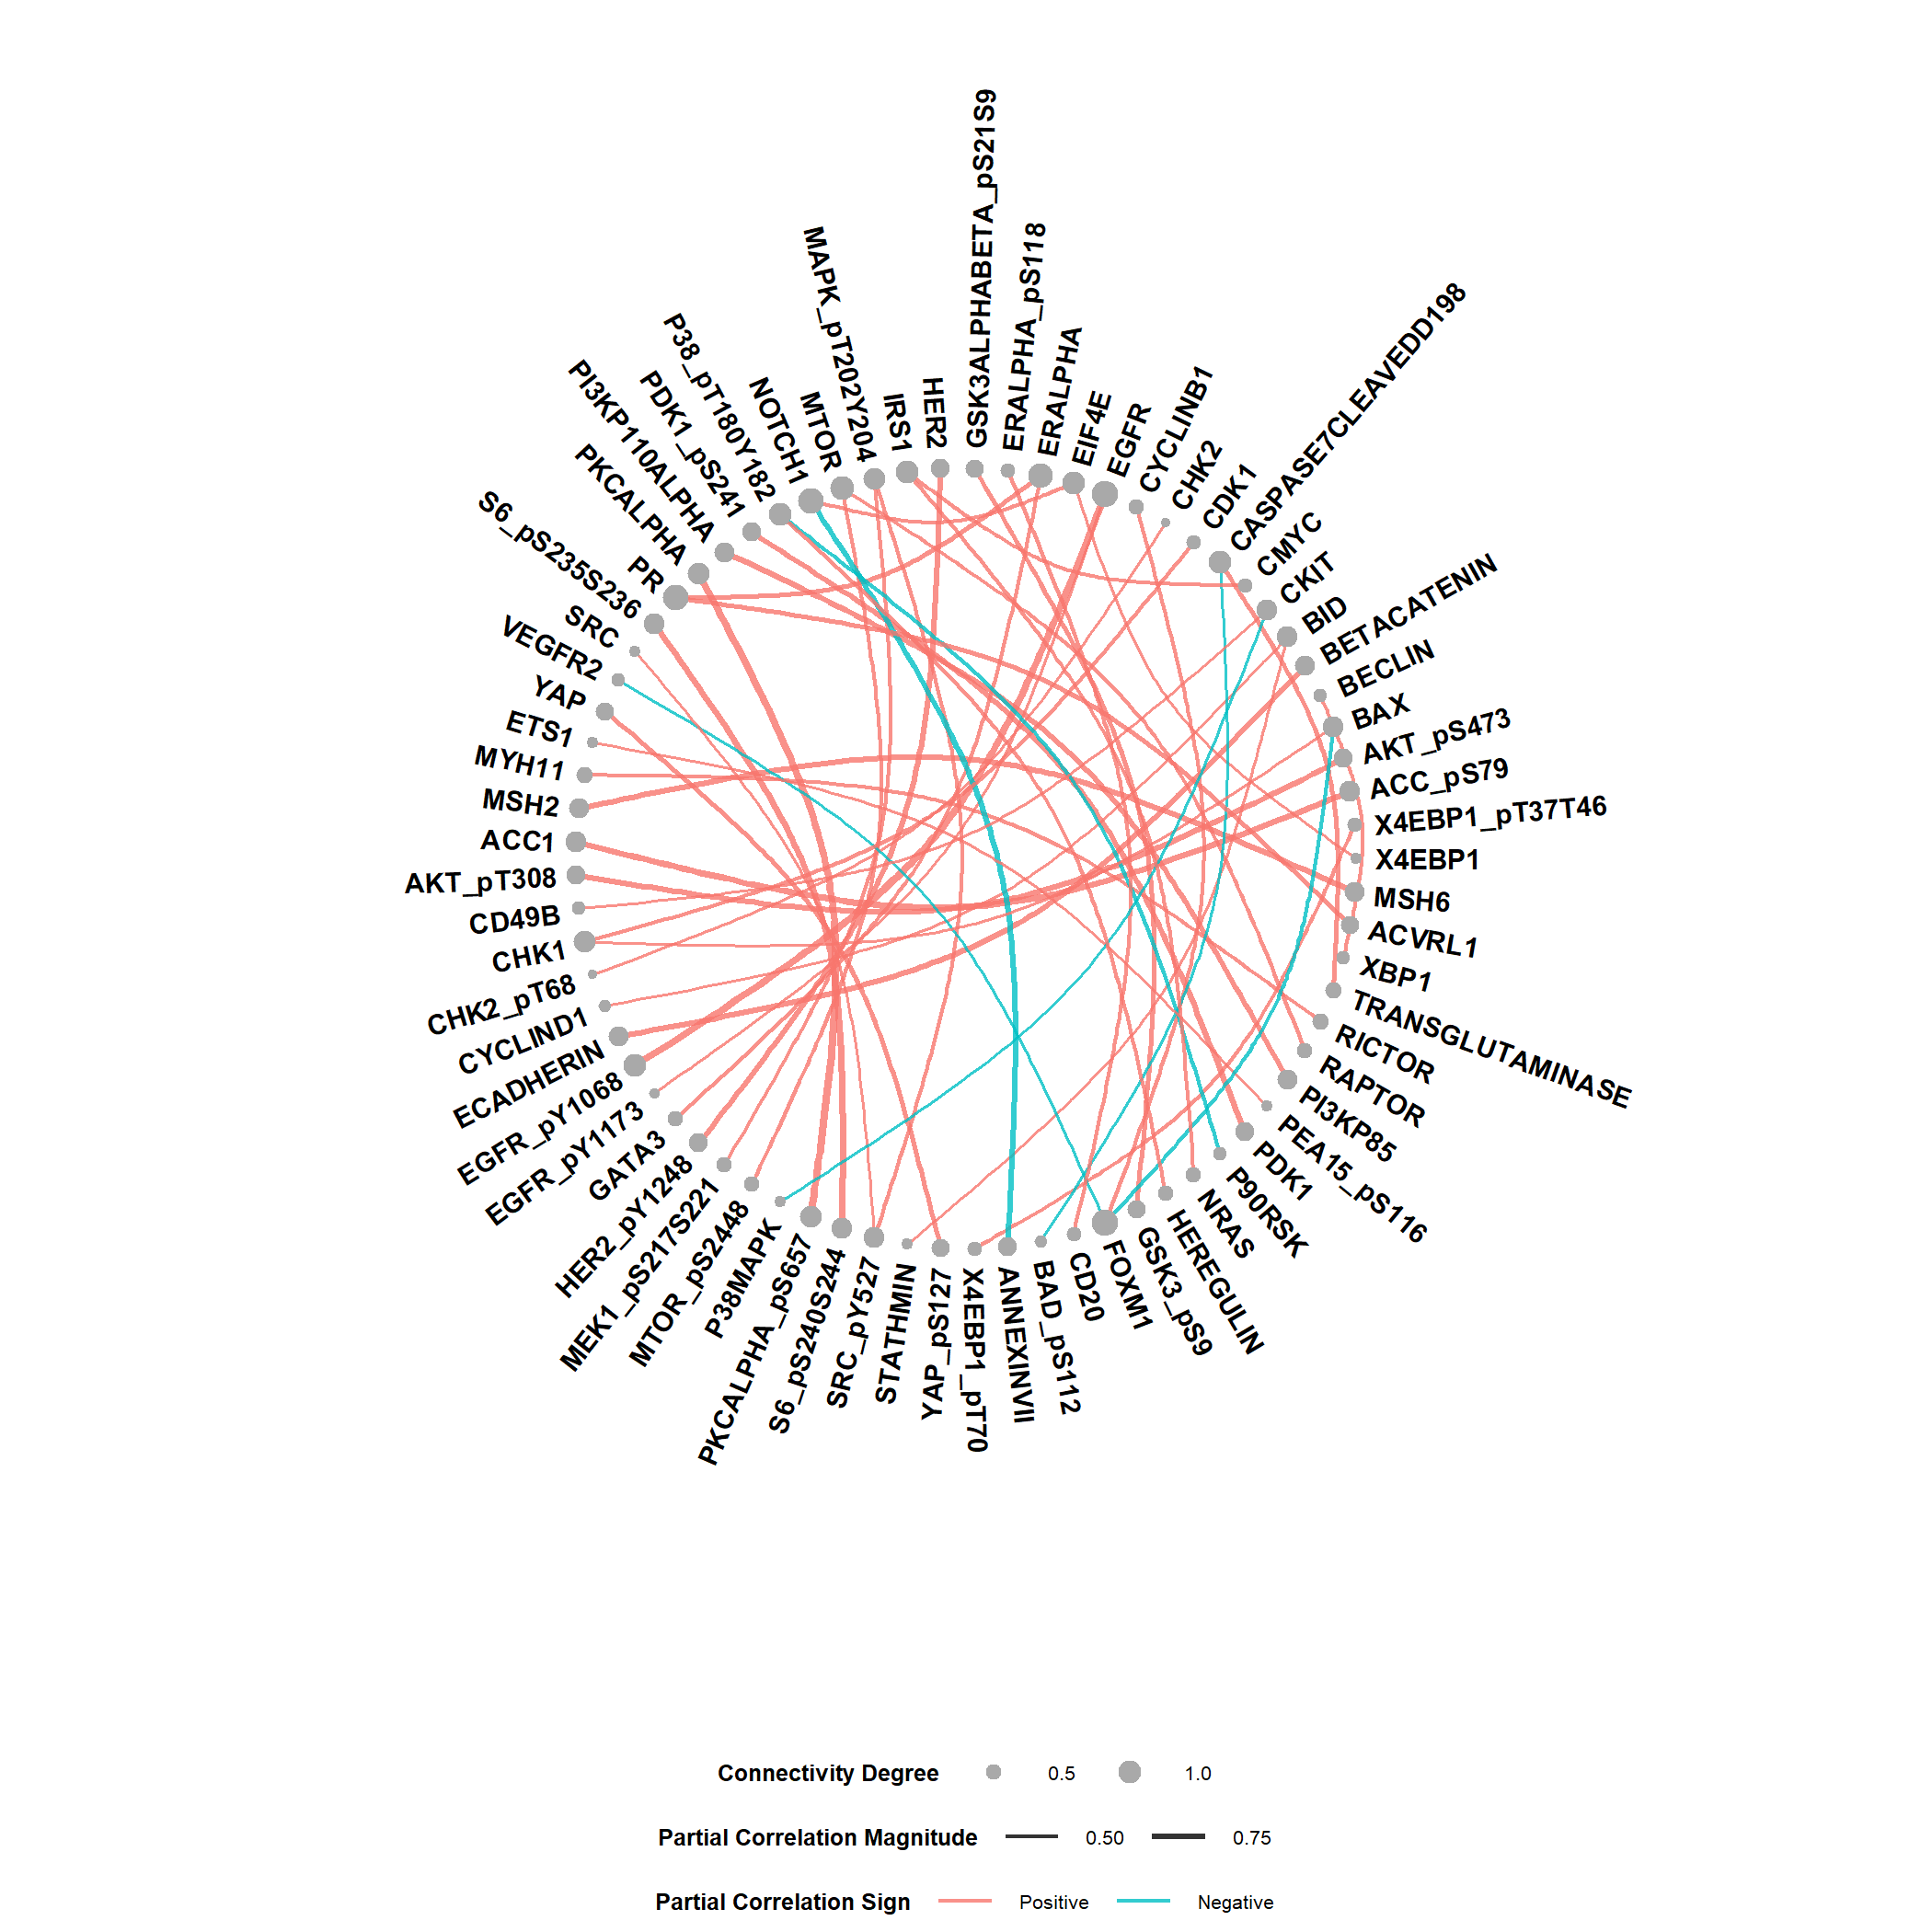
\includegraphics[width=1\linewidth]{man/figures/README-unnamed-chunk-3-1}

\hypertarget{shiny-app-and-tutorial-website}{%
\subsection{Shiny App and Tutorial
website}\label{shiny-app-and-tutorial-website}}

\href{https://bayesrx.shinyapps.io/GraphR/}{Shiny App}

\hypertarget{paper}{%
\subsection{Paper}\label{paper}}

Liying Chen\emph{, Satwik Acharyya}, Chunyu Luo, Yang Ni, Veerabhadran
Baladandayuthapani (2023). GraphR: A probabilistic graphical modeling
framework enables estimation of heterogeneous sample-specific and
spatial genomic networks.

\hypertarget{supplementary-file}{%
\subsection{Supplementary file}\label{supplementary-file}}

\href{https://bookdown.org/bayesrx/graphr_supplementary/}{Supplementary}

\hypertarget{points-to-note}{%
\subsection{Points to note}\label{points-to-note}}

\begin{itemize}
\item
  We recommend to standardize continuous external covariates while
  plugging into the functions.
\item
  It is suggested to maintain \(n/pq > 1\) and efficacy of the method
  increase with high values of \(n/pq\) ratio.
\end{itemize}

\end{document}
